%TODO: more didactics (team work, ..)
%TODO: learning outcomes

% Make nice A4 pages for print:
%\usepackage{pgfpages}
%\pgfpagesuselayout{resize to}[a4paper,border shrink=5mm,landscape]

\beamertemplatenavigationsymbolsempty

\setbeamertemplate{bibliography item}[text]

\usepackage[type={CC},modifier={by-sa},version={4.0}]{doclicense}

\usepackage[utf8]{inputenc}
\usepackage{hyperref}
\usepackage{breakurl}
\usepackage{graphicx}
\usepackage{pgfplots}
\usepackage{pgf}
\usepackage{tikz}
\usetikzlibrary{positioning}
\usetikzlibrary{arrows}
\usetikzlibrary{decorations.markings}
\usetikzlibrary{calc}
\usetikzlibrary{matrix}
\usetikzlibrary{shapes}
\usetikzlibrary{decorations.pathmorphing}
\usetikzlibrary{fit}
\usetikzlibrary{backgrounds}
\usetikzlibrary{plotmarks}
\usepackage{stmaryrd}
\usepackage{listings}
\usepackage{pdflscape}
\usepackage{perpage}
\usepackage{appendixnumberbeamer}

%\usepackage[thmmarks,amsmath,amsthm]{ntheorem} % already included in beamer
\usepackage{thm-restate}

\usepackage[sort&compress,numbers]{natbib}  % to be have \citet, \citeauthor, \citeyear

\MakePerPage{footnote}

\tikzstyle{o}=[r,ppBlue]
\tikzstyle{r}=[thick,rectangle,align=center]
\tikzstyle{t}=[r,ppTrans] %,font=\bfseries]
\tikzstyle{dd}=[densely dashed]
\tikzstyle{n}=[r,ppBlue]
\tikzstyle{p}=[r,ppRed]
\tikzstyle{ppRed}  =[draw=red,  fill=  red!20]
\tikzstyle{ppBlue} =[draw=blue, fill= blue!20]
\tikzstyle{ppGreen}=[draw=green,fill=green!20]
\tikzstyle{ppTrans}=[draw=none, fill=none]

\usetheme{Warsaw}

\useoutertheme[subsection=true]{smoothbars}
%\useoutertheme[subsection=false]{miniframes}

\definecolor{bblue}{HTML}{D7DF01}	% yellow-ish actually, for better black/white printing
\definecolor{rred}{HTML}{C0504D}
\definecolor{ggreen}{HTML}{9BBB59}
\definecolor{ppurple}{HTML}{9F4C7C}
\definecolor{lightgray}{rgb}{0.3,0.3,0.3}
\definecolor{lightergray}{rgb}{0.9,0.9,0.9}
\definecolor{UniBlue}{RGB}{83,121,170}

\DeclareTextFontCommand\textintro{\normalfont\bfseries\itshape} % nice!
\newcommand{\intro}[2][]
{%
	\textintro{#2}%
}
\newcommand{\empha}[2][]
{%
	\emph{#2}%
}

%\theoremstyle{plain}
\newcounter{reqcounter}
\newtheorem{requirement}[reqcounter]{Requirement}

%setbeamercolor{structure}{fg=violet}

\makeatletter
\def\th@task{%
    \normalfont % body font
    \setbeamercolor{block title example}{bg=orange,fg=white}
    \setbeamercolor{block body example}{bg=orange!20,fg=black}
    \def\inserttheoremblockenv{exampleblock}
  }
\makeatother

\theoremstyle{task}
\newtheorem{task}{Task}

\newenvironment{assignment}%
{%\setbeamercolor{background canvas}{bg=violet}%
%\setbeamercolor{structure}{fg=cyan!90!black}%
 \setbeamercolor{frametitle}{bg=orange,fg=white}
\begin{frame}}%
{\end{frame}}%

\AtBeginSection[]{
  \begin{frame}
  \vfill
  \centering
  \begin{beamercolorbox}[sep=8pt,center,shadow=true,rounded=true]{title}
    \usebeamerfont{title}\insertsectionhead\par%
  \end{beamercolorbox}
  \tableofcontents
  \vfill
  \end{frame}
}




\pgfplotsset{compat=1.14}
\author{Markus Raab}


\date{19.6.2019}

\begin{document}

\renewcommand{\enquote}[1]{\emph{``#1''}} % Cannot be done earlier

%%%%%%%%%%%%%%%%%%%%%%%%%%%%%%%
\begin{frame}
	\titlepage
	\doclicenseThis
\end{frame}

\begin{frame}
	\frametitle{Organization}
	Schedule:
	\begin{description}
		\item[15.6.2018:] last corrections of team exercise
		\item[22.6.2018:] oral test
	\end{description}
\end{frame}


\begin{frame}
	\frametitle{Popular Topics}
	\vspace{-0.5cm}
	\begin{multicols}{2}
	\begin{description}
	\color{gray}
	\item[4] validation
	\color{red}
	\item[4] user interface
	\color{gray}
	\item[3] tools (benefits?)
	\item[3] testability
	\item[3] complexity reduction (when conf. needed?)
	\item[3] architectural decisions
	\color{red}
	\item[2] Puppet
	\color{gray}
	\item[2] modularity
	\item[2] environment variables
	\item[2] documentation
	\color{red}
	\item[2] configuration specification
	\color{gray}
	\item[2] command-line args
	\item[2] code generation
	\item[1] variability
	\item[1] self-description
	\item[1] round-tripping
	\item[1] early detection
	\item[1] introspection
	\item[1] dependences
	\item[1] auto-detection
	\item[1] context-awareness
	\color{red}
	\item[1] administrators
	\end{description}
	\end{multicols}
\end{frame}

\begin{frame}
	\frametitle{CM Languages}

	\begin{itemize}[<+-| alert@+>]
	\item What is the relationship to software configuration management (Proteus/PCL)?
	\item[] Build systems may provide configuration management features.
	\item How is it possible to provide referential transparency both for the configuration specification language and for the system itself (NIX, GNU Guix)?
	\item[] By functional languages and file system (layouts).
	\item Which notations for CM exist?
	\item[] Text,  Graphical (UML), Semi-structured, Key-value, Structured
	\end{itemize}
\end{frame}



%%%%%%%%%%%%%%%%%%%%%%%%%%%%%%%%%%%%%%%%%% 
\section{User View}

\subsection{}

\begin{frame}
	\frametitle{User View}

	Who is the user of CM?

	\begin{itemize}[<+-| alert@+>]
	\item End Users?
	\item Developers (devs)?
	\item System Administrators (admins)?
	\end{itemize}
\end{frame}

\begin{frame}
	\frametitle{System Administrator Research}

	\begin{itemize}[<+-| alert@+>]
	\item Interest of understanding administrators emerged around 2002~\cite{anderson2002researching}.
	\item Typical methods are surveys, diary studies, interviews and observations (ethnographic field studies).
	\item Field studies also done in industry \cite{barrett2004field}.
	\item Barrett \cite{barrett2003system} tried to initiate a workshop at CHI 2003 to draw the attention of the HCI community towards system administration.
	\item The workshop was already dropped in the next year.
	\item The tenor is that ``tools ... are not well aligned''~\cite{haber2007design}.
	\item Research mainly looks at pre-CM. Manual administration is still standard (Source: e.g., Luke Kanies).
	\end{itemize}
\end{frame}


\begin{frame}
	\frametitle{CM research}

	In the meanwhile at Large Installation System Administrator Conference (LISA):

	\begin{itemize}[<+-| alert@+>]
	\item began as CFengine Workshop at LISA 2001
	\item CM workshop by Paul Anderson~\cite{anderson2002researching}
	\item in LISA 2003 an informal poll asked about CM tools: \\
	 	the only user of each tool in the room at the time was its author~\cite{burgess2006modeling}
	\item it is easy to invent CM tools (and configuration file formats)
	\item it is difficult to make it useful beyond your own goals
	\end{itemize}
\end{frame}

\begin{frame}
	\frametitle{Tasks}

	What do system administrators do?

	\begin{itemize}[<+-| alert@+>]
	\item keep our infrastructure running
	\item coordinate
	\item do backups
	\item manage hardware
	\item do inventory
	\item install applications
	\item manage security
	\item configure applications
	\item troubleshoot
	\item $\implies$ the unsung heroes!
	\end{itemize}
\end{frame}


\begin{frame}
	\frametitle{7 people, 1 command-line~\cite{barrett2004field}}

	\begin{itemize}[<+-| alert@+>]
	\item system administrator misunderstood problem \\ (had a wrong assumption)
	\item 7 people sought attention and trust, competing to tell the admin what to do
	\item due to wrong assumption the admin communicated to everyone, people could not help
	\item there were several instances in which the admin ignored or misinterpreted evidence of the real problem
	\item eventually someone else solved the problem: admin confused ``from''/``to'' port in the settings and firewall blocked requests
	\end{itemize}
\end{frame}

\begin{frame}
	\frametitle{other cases~\cite{barrett2004field}}

	\begin{itemize}[<+-| alert@+>]
	\item lost semicolon: execution of script failed due to missing semicolon, then they tried to delete a non-existent table.
	\item crontab: onltape/ofltape confused because of discussion about offline backup (although an online backup should be performed).
	\item crit sit: many system administrators competed against each other trying to write a simple script. The crit sit continued for two weeks.
	\end{itemize}
\end{frame}


\begin{frame}
	\frametitle{\citet{haber2007design}}

	Later \citet{haber2007design} repeated an ethnographic field study.
	The stories are similar to \citet{barrett2004field}.
	Their study was also conducted in the same company.
	They created personas:

	\begin{itemize}
	\item database administrator
	\item web administrator
	\item security administrator
	\end{itemize}
\end{frame}



\begin{frame}
	\frametitle{Database Administrator~\cite{haber2007design}}

	\begin{itemize}[<+-| alert@+>]
	\item frequent contact via phone, e-mail and IM
	\item needs to work on weekends
	\item pair-programming for new tasks
	\item typical errors: stopping wrong database process
	\end{itemize}
\end{frame}

\begin{frame}
	\frametitle{Web Administrator~\cite{haber2007design}}

	\begin{itemize}[<+-| alert@+>]
	\item crit sit
	\item deploying new Web applications
	\item about 20-400 steps to deploy an application
	\item moving from test to production done by hand
	\end{itemize}
\end{frame}

\begin{frame}
	\frametitle{Security Administrator~\cite{haber2007design}}

	\begin{itemize}[<+-| alert@+>]
	\item gets emails on suspicious activities
	\item multi-user chat
	\item ad-hoc scripts
	\end{itemize}
\end{frame}


\begin{frame}
	\frametitle{\citet{haber2007design}}

	\begin{itemize}[<+-| alert@+>]
	\item ``if data is lost...that is when you write your résumé.''
	\item \p{90} is spent with communicating with other admins
	\item \p{20} of the time is spent in diversions~\cite{barrett2004field}
	\item \p{20} of the time people communicated about \emph{how to communicate}~\cite{barrett2004field}
	\item \p{6} is gathering information and running commands
	\item quality control: monitoring found that non-functional service was down two days
	\item CLIs were generally preferred
	\item configuration and log files are scattered, poorly organized and often used inconsistent terminology
	\end{itemize}
\end{frame}


\begin{frame}
	\frametitle{Findings \cite{barrett2004field}}

	\begin{itemize}[<+-| alert@+>]
	\item syntax checking is essential
	\item replicating actions (e.g., to production) is error-prone
	\item undo not available
	\item do not assume a complete mental model (``if understand the system is a prerequisite [...], we are lost'')
	\item do not assume programming skills (only \p{35} reported having a bachelor's degree)
	\item trust in CLI tools but little trust in GUIs (is the information up-to-date?)
	\item errors while executing scripts lead to inconsistent state, rerunning often does not work (if not idempotent)
	\end{itemize}
\end{frame}

\begin{frame}
	\frametitle{Design Principles \cite{haber2007design}}

	Many design principles for tools were given~\cite{haber2007design}:

	\begin{itemize}[<+-| alert@+>]
	\item configuration and logs should be displayed in a uniform way
	\item APIs/plugins for tools should be provided
	\item errors in configuration need to be discovered quickly
	\item confusion of similar settings should be avoided: add links, explain interactions
	\item provide means of comparing configuration settings
	\item provide consistent profiles of information
	\item both transient and persistent settings should be visible
	\item when errors occur: always display which changes have been made (modern approach is idempotence)
	\end{itemize}
\end{frame}





%%%%%%%%%%%%%%%%%%%%%%%%%%%%%%%%%%%%%%%%%% 
\section{Configuration Management}

\subsection{}

\begin{frame}
	\frametitle{Apply to CM}

	What can we learn from system administration research?

	\setbeamersize{description width=1cm}
	\begin{description}[<+-| alert@+>] %[leftmargin=0cm] %TODO: move left
	\item[$+$] intensive review process catches errors
	\item[$-$] collaboration ineffective
	\item[$-$] context/situational awareness is essential
	\item[$+$] precise editing of configuration files works well
	\item[$-$] global optimizations difficult
	\item[$+$] self-written tools are very efficient
	\end{description}

	\pause[\thebeamerpauses]  %  show after \begin{itemize}[<+->]

	\begin{alertblock}{Idea}
	Replicate parts that work well, automate error-prone parts.
	\end{alertblock}
\end{frame}

\begin{frame}
	\frametitle{Precise Editing}

	Partial modifications (precise editing) is natural for humans. \\
	It ensures preservations of (potentially security-relevant!) defaults. \\
	In CM, however, following methods are used:

	\setbeamersize{description width=1cm}
	\begin{itemize}[<+-| alert@+>] %[leftmargin=0cm] %TODO: move left
	\item embed shell commands to do the work
	\item replace full content of configuration files
	\item replace full content of configuration files with templates
	\item line based manipulation (e.g., file\_line): match line and replace it
	\item Augeas/XML: match a key with XPath and replace it
	\item Elektra: set the value of a key
	\end{itemize}
\end{frame}

\begin{frame}[fragile]
	Key/value access in puppet-libelektra:

	\begin{code}[morekeywords={kdbkey,kdbmount,ensure,value},gobble=4]
	kdbmount {'system/sw/samba':
		ensure => 'present',
		file => '/etc/samba/smb.conf',
		plugins => 'ini'
	}
	kdbkey {'system/sw/samba/global/workgroup':
		ensure => 'present',
		value => 'MY_WORKGROUP'
	}
	kdbkey {'system/sw/samba/global/log level':
		ensure => 'absent'
	}
	\end{code}

	Uniqueness of keys is essential.
	Ideally, applications already mount their configuration at installation.
\end{frame}


\begin{frame}
	\frametitle{Apply to CM}

	Elektra's goals are that it should:

	\begin{itemize}[<+-| alert@+>]
	\item be easy to develop new high-level tools
	\item support manual workflows and scripts
	\item support precise editing:\\ only change the configuration value as specified
	\item provide a language for both devs and admins
	\end{itemize}

	\pause[\thebeamerpauses]  %  show after \begin{itemize}[<+->]

	Admins/devs still need to:

	\begin{itemize}[<+-| alert@+>]
	\item reduce the configuration space
	\item intensively review and improve the specifications
	\item test (and debug) configuration settings
	\end{itemize}
\end{frame}

\begin{frame}[fragile]
	Key/value specifications in puppet-libelektra:

	\begin{code}[morekeywords={kdbkey,ensure,value},gobble=4]
	kdbkey {'system/sw/samba/global/log level':
		ensure => 'present',
		value => 'MY_WORKGROUP',
		check => {
			'type' => 'short',
			'range' => '0-10',
			'default' => '1',
			'description' => 'Sets the amount of log/
				debug messages that are sent to the
				log file. 0 is none, 3 is consider-
				able.'
	}
	\end{code}

	Ideally, applications already specify their settings.
\end{frame}

\begin{frame}
	\frametitle{Key/Values Revisited}

	Decide about \textbf{changeability} per key:

	\begin{itemize}[<+-| alert@+>]
	\item Who is responsible (end user, packages, admin manual or CM).
	\item In which namespaces apps search the key (cascading lookup).
	\item Who can see it (visibility).
	\item Who can edit it (admin, end user, both).
	\item Which configuration values are allowed (validation).
	\end{itemize}

	\pause[\thebeamerpauses]  %  show after \begin{itemize}[<+->]

	\begin{alertblock}{Changeability}
	Ownership of every key must be very clear and documented.
	\end{alertblock}
\end{frame}

\begin{frame}[fragile]
	Key/value specifications in puppet-libelektra:

	\begin{code}[morekeywords={kdbkey,ensure,value},gobble=4]
	kdbkey {'spec/xfce/pointers/Mouse/RightHanded':
		ensure => 'present',
		check => {
			'namespaces/#0' => 'user',
			'namespaces/#1' => 'system',
			'visibility' => 'important',
			'default' => 'false',
			'check/type' => 'boolean'
	}
	\end{code}

	Ideally, applications already specify their settings.
\end{frame}

\begin{frame}
	\frametitle{Layers of Abstractions}

	Recursively define useful abstractions (meta-levels):

	\begin{itemize}[<+-| alert@+>]
	\item Bits in (configuration) files and memory
	\item Key/value view of configuration settings
	\item Goals/specifications of settings per node and instantiations of modules
	\vspace{1em}
	\item CM code to instantiate settings in the whole network
	\item Global optimization: allocation of nodes and decision regarding topology in the whole network
	\item Global goals/specifications of the whole network
	\end{itemize}
\end{frame}

\begin{assignment}
	\begin{task}
	Break.
	\end{task}
\end{assignment}

\begin{frame}
	\frametitle{Design Rules~\cite{burgess2006modeling}}

	\begin{itemize}[<+-| alert@+>]
	\item Factor processes into containers to avoid overlaps in settings.
	\item Maintain clear separation of ownership (for every key).
	\item Specify replicated settings in a single source (use links and derivations).
	\item Document all remaining overlaps (in the specification).
	\item The manageability of settings is reduced by the number of possible configuration values.
	\item Do not separate configuration management and monitoring.
	\end{itemize}
\end{frame}


\begin{frame}
	\frametitle{Open Topics}

	\begin{itemize}[<+-| alert@+>]
	\item global optimizations/self-healing
	\item configuration integration
	\item safe migrations of settings and data
	\item collaboration
	\item management (including knowledge)
	\item centralized vs.\ distributed
	\end{itemize}
\end{frame}


\begin{frame}
	\frametitle{Conclusion}

	\begin{itemize}[<+-| alert@+>]
	\item create stateless transactions with key/values (get/set)
	\item be aware of the specifications, solving CM is solving constraints
	\item do not design around tools but design tools around you
	\item be brave and remove all configuration settings you can
	\item use all help you can get: e.g.\ build tools, preseeding, installer automation, virtualization, package managers, distributions
	\item complexity in CM vs.\ complexity in applications' specification
	\item modularity is essential for validation and legacy support
	\item artifact generation improves consistency and type safety
	\end{itemize}
\end{frame}






%%%%%%%%%%%%%%%%%%%%%%%%%%%%%%%%%%%%%%%%%% 
\section{Recapitulation}

\subsection{}

\begin{frame}
	\frametitle{Introspection (Recapitulation)}
	\begin{task}
	What is internal and external specification?
	What is introspection?
	\end{task}

	\pause
	\vspace{1em}

	\begin{itemize}
	\item \textit{internal}: within applications' source code
	\item \textit{introspection}: unified get/set access to (meta*)-key/values
	\item access via applications, CLI, GUI, web-UI, ...
	\item access via any programming language (similar to file systems)
	\item GUI, web-UI can semantically interpret metadata
	\item assemble modular parts (validation, logging, \dots)
	\item needed as communication between producers and consumers
	\item essential for \intro[no-futz computing]{no-futz computing}~\citet{holland2001nofutz}
	\end{itemize}
\end{frame}

\begin{frame}
	\frametitle{KeySet (Recapitulation)}

	The common data structure of Elektra:
	\vspace{1cm}

	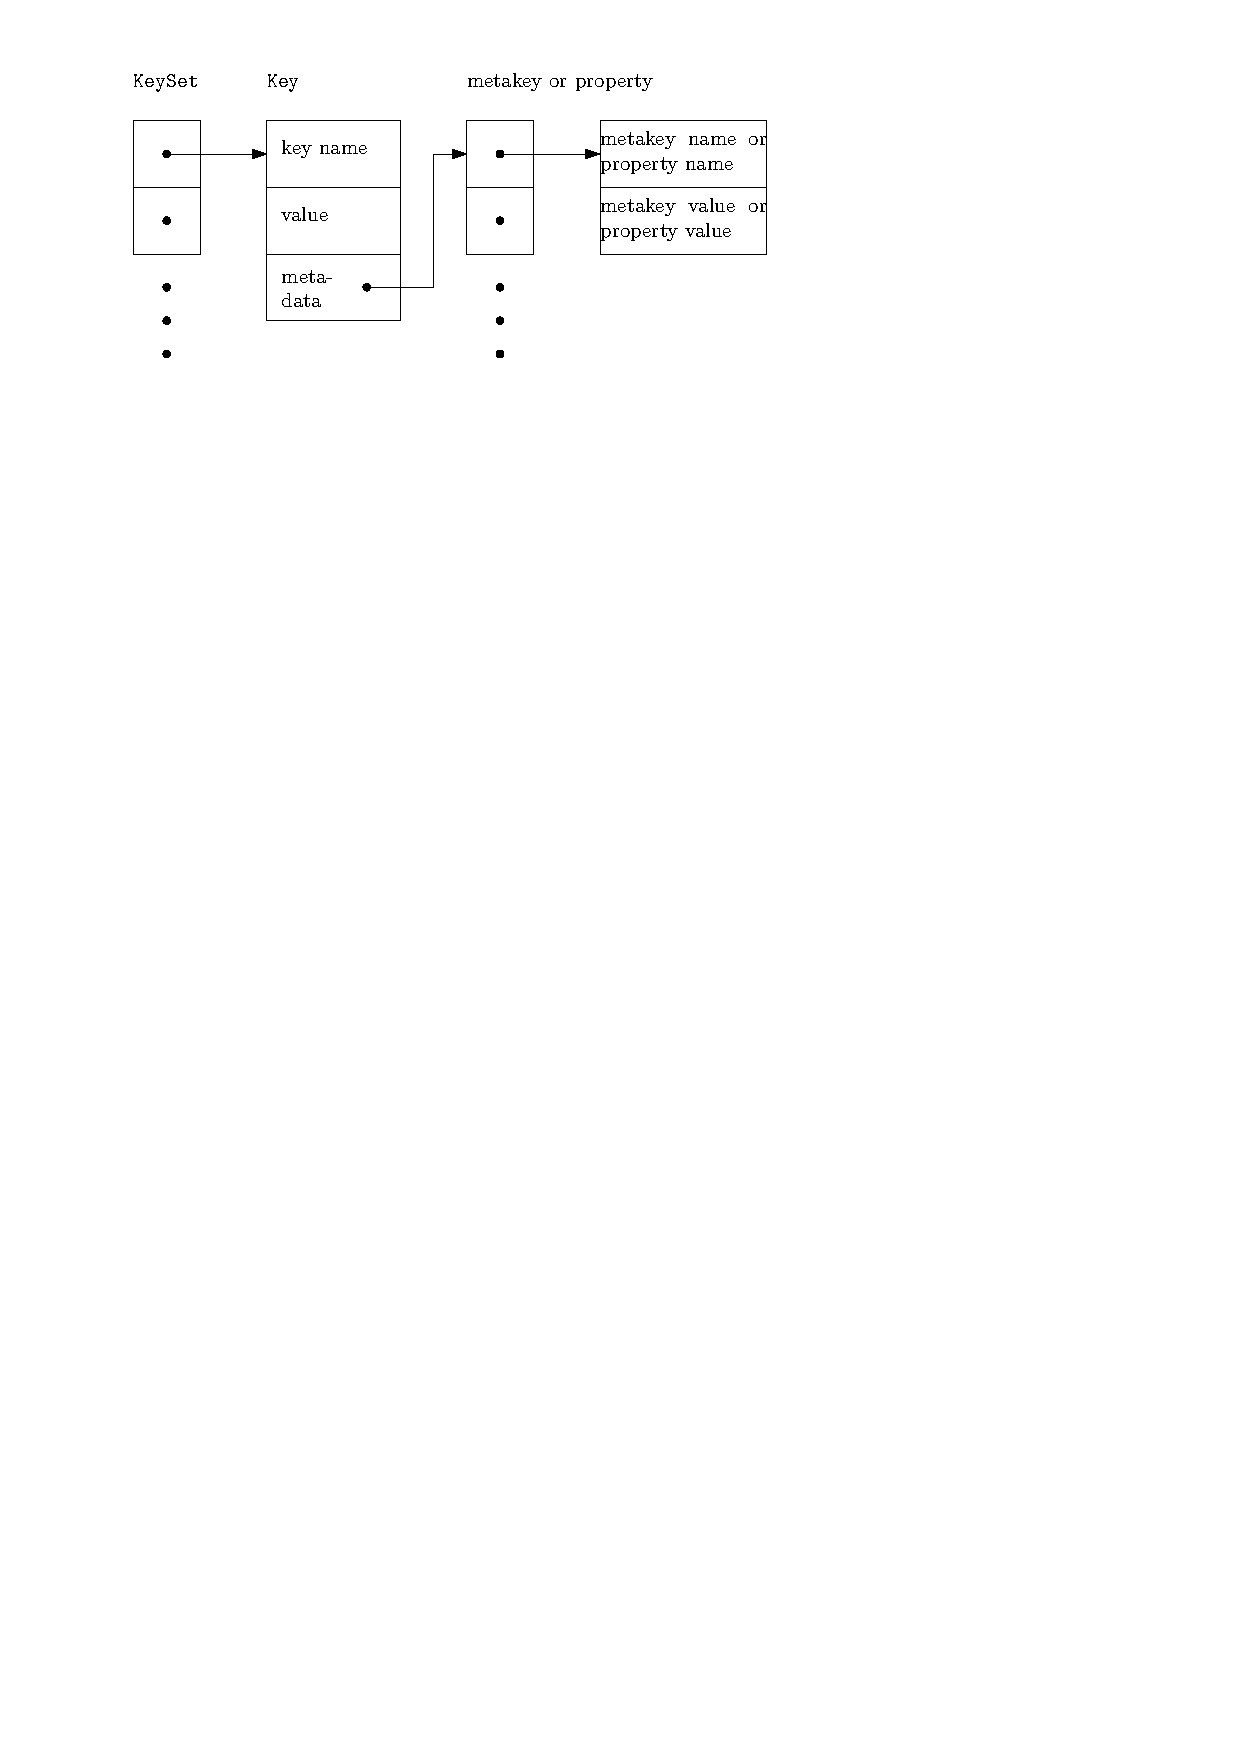
\includegraphics{keyset}
\end{frame}

\begin{frame}
	\frametitle{Testing (Recapitulation)}
	\begin{task}
	What do we want to test?
	\end{task}

	\pause

	\begin{itemize}
	\item That settings do what they should (devs and admins)
	\item That settings are properly validated (devs~\cite{xu2013blame})
	\item Regression tests (devs~\cite{qu2008configuration})
	\vspace{1em}
	\item Are all settings implemented? (devs)
	\item Are all settings used in tests? (devs)
	\item Are there unused settings in the code? (devs)
	\item Do the chosen settings work? (admins)
	\end{itemize}
\end{frame}

\begin{frame}
	\frametitle{Early detection (Recapitulation)}
	\begin{task}
	When do we want to detect misconfiguration?
	\end{task}

	\pause

	Phases when we can detect misconfigurations:
	\begin{itemize} %[<+-| alert@+>]
	\item Compilation stage in configuration management tool
	\item Writing configuration settings on nodes
	\item Starting applications (load-time)
	\item When configuration setting is actually used (run-time)
	\end{itemize}

	\pause[\thebeamerpauses]

	\begin{alertblock}{Problem}
	Earlier versus more context.
	\end{alertblock}
\end{frame}

\begin{frame}
	\frametitle{Notification (Recapitulation)}

	\begin{task}
	Why do we need notification?
	\end{task}

	\pause

	\begin{enumerate}
	\item to keep transient and persistent configuration settings always in sync~\cite{jin2014configurations}
	\item to avoid polling of configuration settings
	\item to better integrate into already existing mechanisms (main loops)\footnote{Is one of the main reasons why most framework already integrate configuration settings.}
	\end{enumerate}

	\ExecuteMetaData[../book/motivation.tex]{req-consistency}
\end{frame}

\begin{frame}
	\frametitle{Cascading (Recapitulation)}

	\begin{task}
	What is cascading configuration?
	\end{task}
	\vspace{1em}

	\pause

	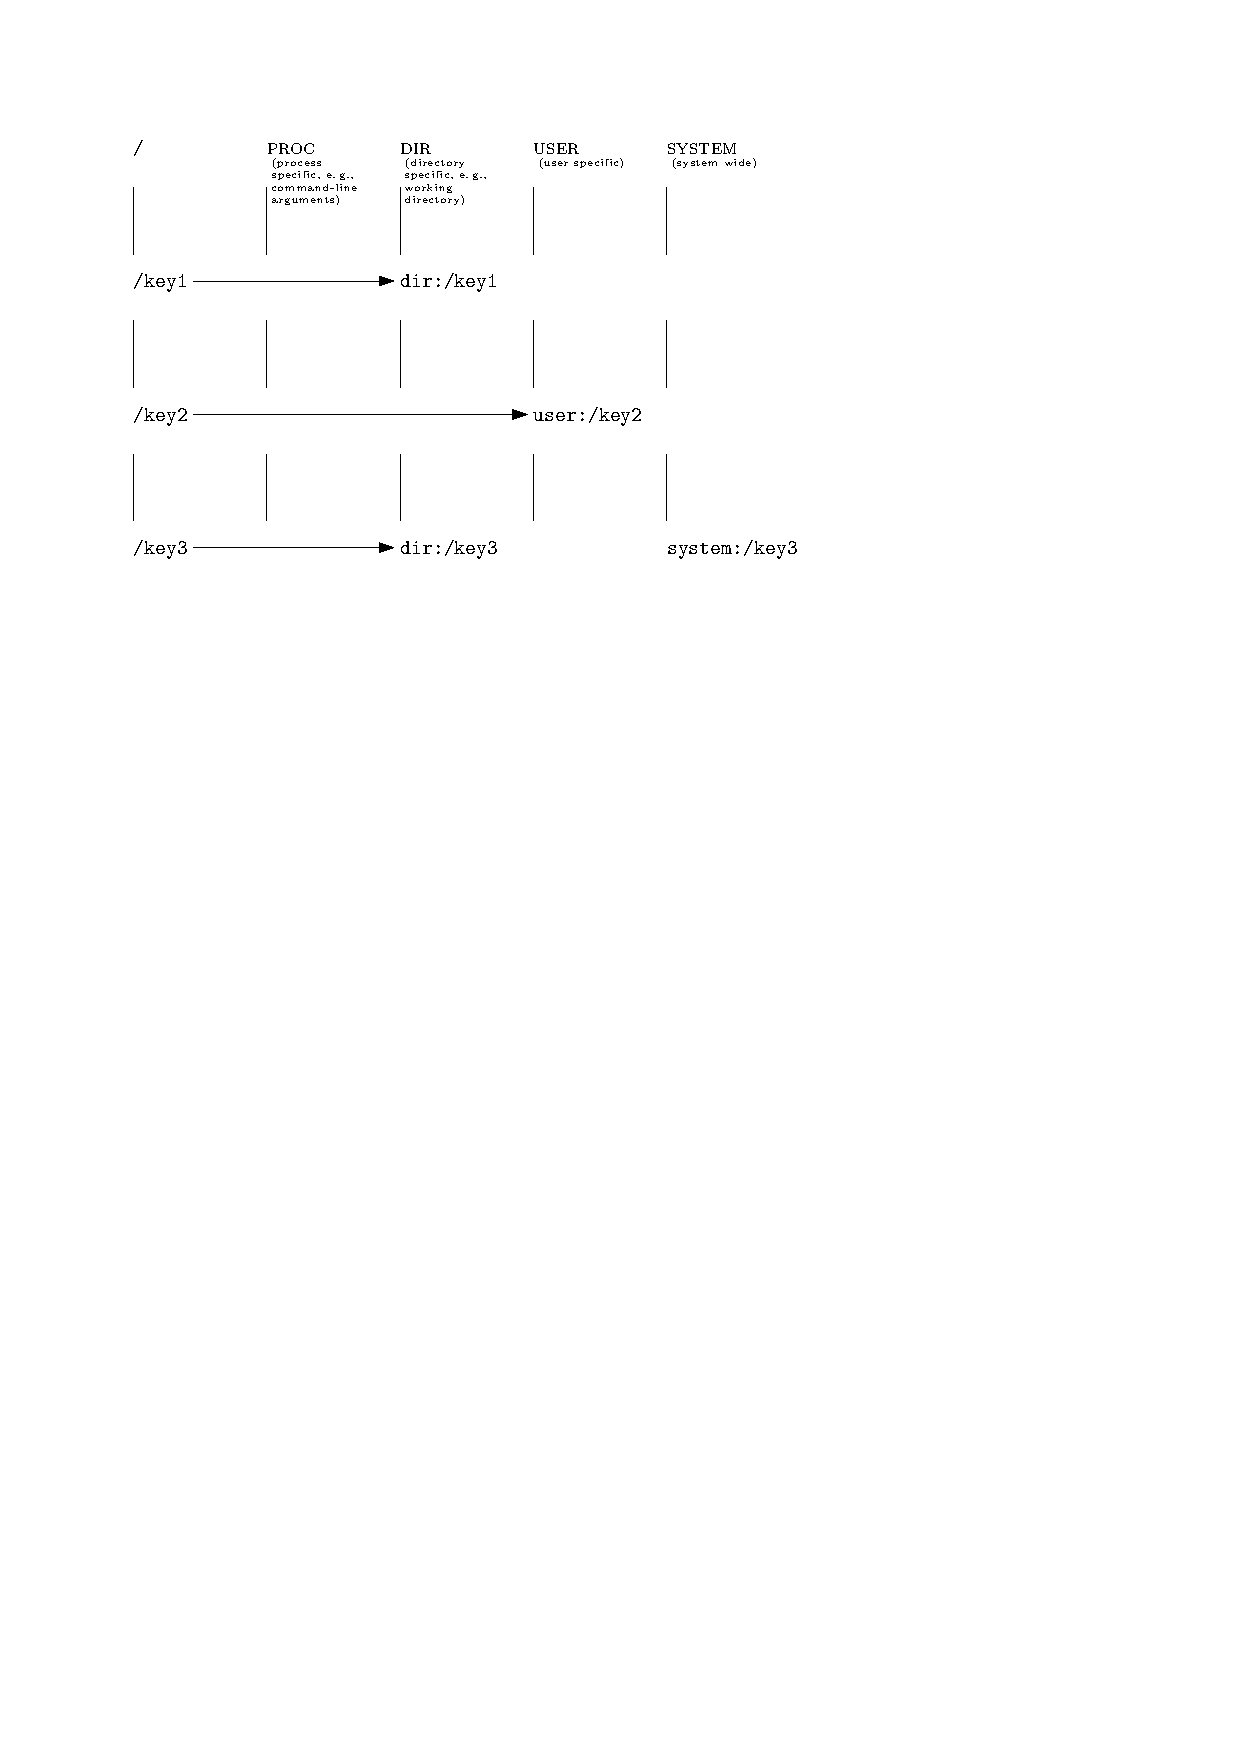
\includegraphics[scale=0.7]{cascading}
\end{frame}

\begin{frame}
	\frametitle{Contextual Values (Recapitulation)}

	\begin{task}
	What are contextual values?
	\end{task}

	\pause

	\ExecuteMetaData[../book/background.tex]{contextual-values}
\end{frame}

\begin{frame}
	\frametitle{Introspection vs.\ Code Generation (Recapitulation)}

	\begin{task}
	Advantages/Disadvantages of key database (vs.\ code generation)?
	\end{task}

	\pause

	\setbeamersize{description width=1cm}
	\begin{description} %[leftmargin=0cm] %TODO: move left
	\item[$+$] specification can be updated live on the system without recompilation
	\item[$+$] tooling has generic access to all specifications
 	\item[$+$] new features the key database (e.g., better validation) are immediately available consistently
	\item[$-$] less techniques for performance improvements
	\item[$-$] contextual values cannot be used if context differs within same thread
	\end{description}

	\begin{alertblock}{Implication}
	We generally prefer introspection, except for a very thin configuration access API.
	\end{alertblock}
\end{frame}

\begin{frame}
	\frametitle{Definition Configuration Management (Recapitulation)}

	\begin{task}
	What is Configuration Management?
	\end{task}

	\pause

	\begin{itemize}
	\item is a discipline in which configuration (in the broader sense) is administered.
	\item makes sure computers are assembled from desired parts and the correct applications are installed.
	\item has means to describe the desired configuration of the whole managed system.
	\item ensures that the execution environment of installed applications is as required.
	\end{itemize}
\end{frame}

\begin{frame}
	\frametitle{Possible Benefits of CM (Recapitulation)}

	\begin{task}
	What are the goals of Configuration Management?
	\end{task}

	\pause

	\begin{itemize} %[<+-| alert@+>]
	\item The same goals scripts have: \\
		Documentation, Customization, Reproducability
	\item Declarative description of the system \\
		Single Source of Truth 
		(Infrastructure as Code~\cite{waldemar2013testing})
	\item Less configuration drift
	\item Error handling
	\item Pull vs.\ Push
	\item Reusability
	%\item (Resource) Abstractions
	\end{itemize}
\end{frame}

\begin{frame}
	\frametitle{Types of Specifications (Recapitulation)}

	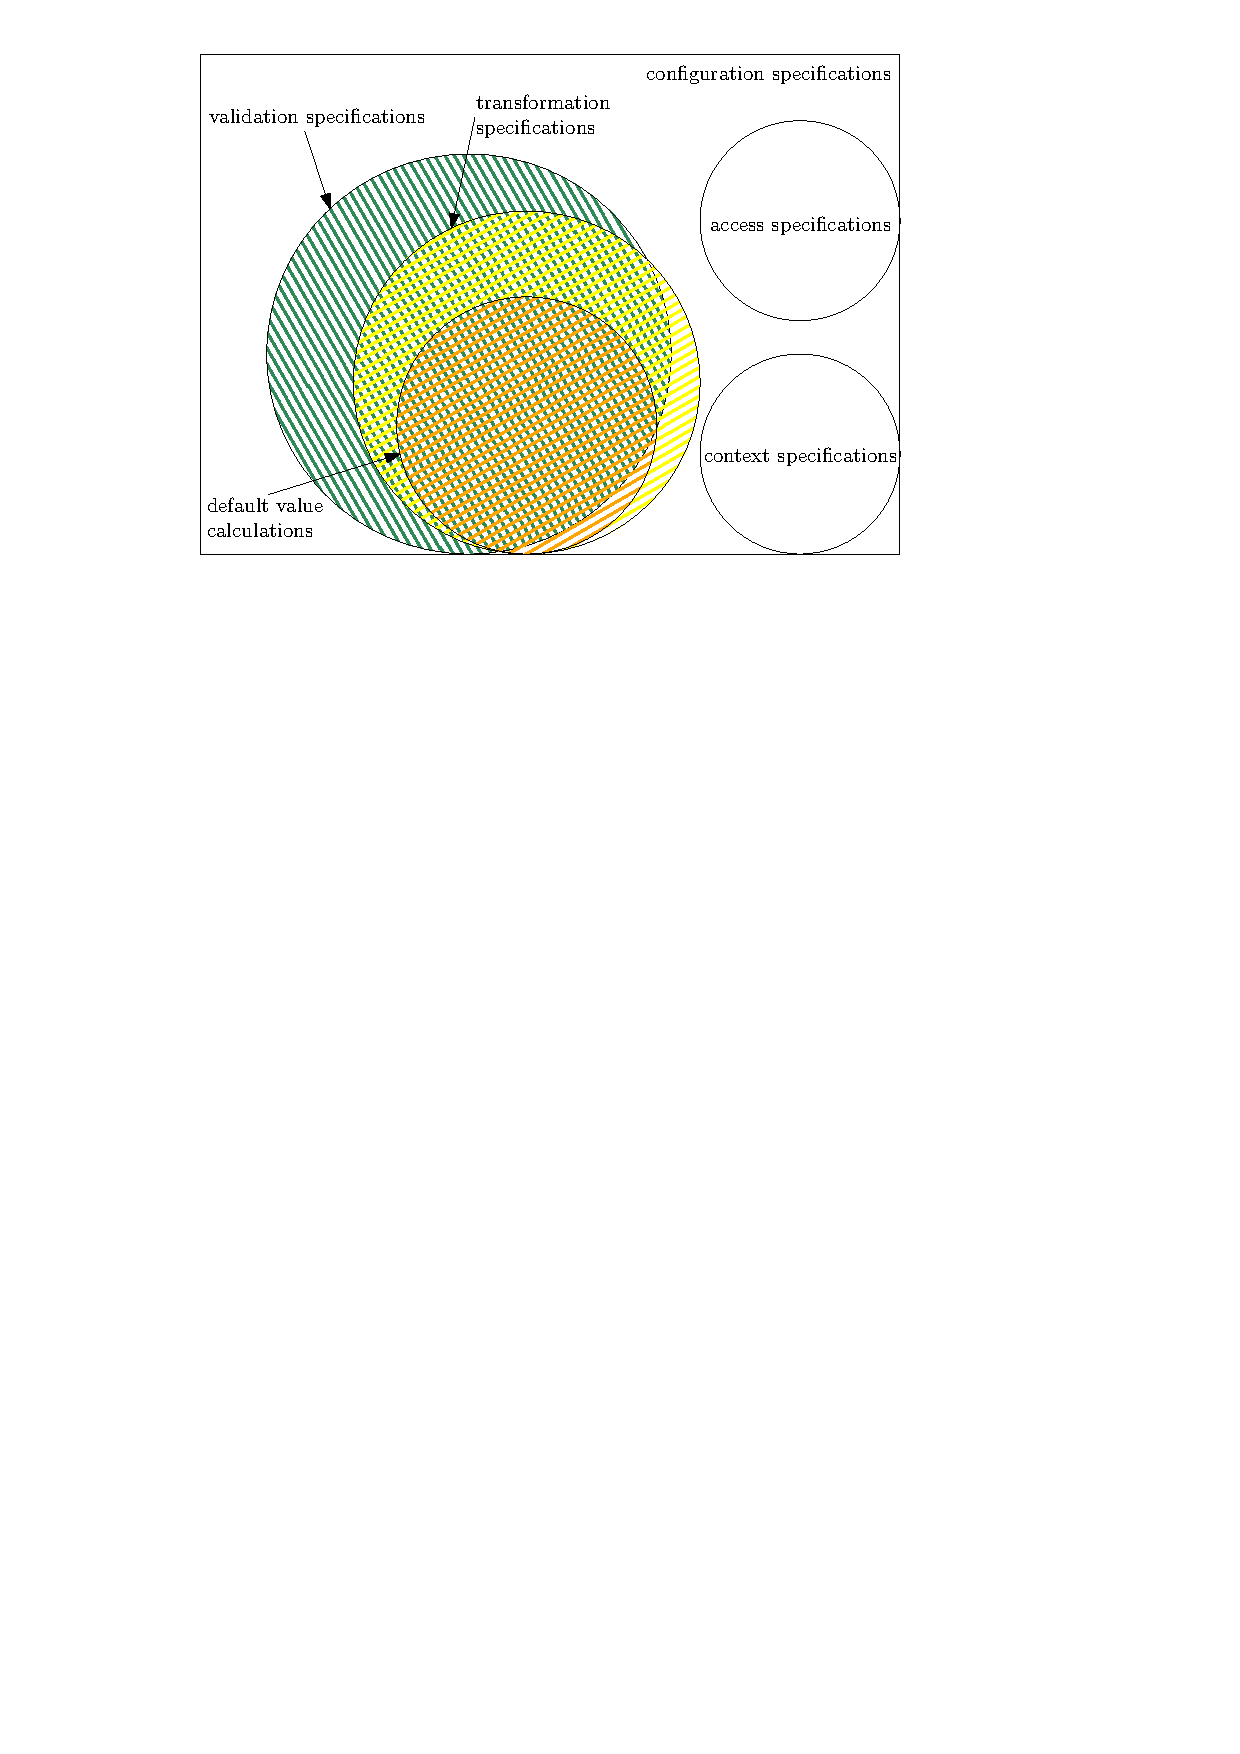
\includegraphics[scale=0.8]{specifications}
\end{frame}


\begin{frame}
	\frametitle{Configuration Specification (Recapitulation)}

	\begin{task}
	How can we combine configuration specifications and configuration management?
	\end{task}

	\pause

	\begin{itemize} %[<+-| alert@+>]
	\item configuration settings are simply an instantiation of the configuration specifications.
		Code describing the instantiation is \textbf{CM code}.
	\item configuration design is explicit (like transformations and default values) and can help while writing CM code.
	\item CM code can even be generated from the specification.
	\item access specifications make access trivial via uniform interface.
	\item visibility and similar techniques may help dealing with complexity.
	\end{itemize}
\end{frame}

\begin{frame}
	\frametitle{Configuration Drift (Recapitulation)}

	\begin{task}
	What is configuration drift? What are its causes?
	\end{task}

	\pause

	Are derivations of the ``Single Source of Truth'' (the CM code).

	Caused by:

	\begin{itemize} %[<+-| alert@+>]
	\item manual configuration changes by administrators
	\item manual configuration changes by end users
	\item differences in updates (e.g., skipped or failed updates)
	\item failed attempts to change configuration
	\item applying different versions of CM code
	\item \dots
	\end{itemize}


\end{frame}

\begin{frame}
	\frametitle{Idempotence (Recapitulation)}

	\begin{task}
	What is idempotent, self-describing, round-tripping configuration?
	\end{task}

	\pause


	\begin{description}
	\item[Idempotent]
	yield the same configuration with any number of applications from CM code ($n\ge1$)~\cite{waldemar2013testing}:
	\[
		f(f(x))=f(x)
	\]
	needed to guarantee repeatability

	\item[Self-describing]
	means that from the configuration file alone we are able to derive the correct data structure~\cite{wadler2003xml}.

	\item[Round-tripping]
	means that if a data structure is serialized and then parsed again, we end up with an identical data structure~\cite{wadler2003xml}.
	\end{description}

	The data structure could be a KeySet.
\end{frame}

\begin{frame}
	\frametitle{Checking Configurations (Recapitulation)}

	\begin{task}
	Which properties of configuration settings can be checked?
	\end{task}

	\pause

	\begin{itemize} %[<+-| alert@+>]
	\item structure
	\item values (data types)
	\item constraints
	\item semantic checks (e.g., IP, folder)
	\item domain-specific checks (e.g., databases)
	\item requirements (suitable configurations)
	\item context (context-aware configurations)
	\end{itemize}
\end{frame}

\begin{frame}
	\frametitle{Popular CMs today (Recapitulation)}

	\begin{itemize} %[<+-| alert@+>]
	\item CFengine
	%\item Bcfg2
	\item LCFG
	\item Config Mgmt
	\item Quattor
	\item Puppet
	\item Chef
	\item Ansible (Talk next week)
	\item SaltStack (Talk today)
	\item Rudder
	\item Spacewalk
	\end{itemize}
\end{frame}

\begin{frame}
	\frametitle{Elektra (Recapitulation)}

	\begin{task}
	What is Elektra?
	\end{task}

	\pause

	\begin{itemize}
	\item is not only a key database but a specification language to describe a key database
	\item plugins implement the specification (could be distributed but focus is configuration files)
	\item is library based (no single point of failure, no distributed coordination needed)
	\item supports transactions (persisting whole KeySets at once)
	\item supports integration of existing configuration settings
	\end{itemize}
\end{frame}


\begin{frame}
	\frametitle{Error Messages (Recapitulation)}

	\begin{task}
	What needs to be considered when designing error messages?
	\end{task}

	\pause

	\begin{itemize} %[<+-| alert@+>]
	\item error messages are often the sole data source for admins
	\item configuration design first: avoid errors if possible
	\item error messages should not leak internals~\cite{brown1983error}
	\item ``edit here mentality'': do not point to correct statements~\cite{marceau2011mind}
	\item Precisely locate the cause (and do not report aftereffects)
	\item Personification~\cite{lee2011personifying}
	\item give context: providing enough information vs.\ not overwhelming the user~\cite{wrenn2017error}
	\end{itemize}
\end{frame}

\begin{frame}
	\frametitle{Context for error messages (Recapitulation)}

	\begin{task}
	What should error messages contain?
	\end{task}

	\pause

	\begin{itemize} %[<+-| alert@+>]
	\item pin-point key (which also pin-points to the specification)
	\item repeat relevant parts of values and the specification
	\item show mountpoint (to make relative keys unique)
	\item show file name and line number
	\item ? show module and source code lines (for bugs)
	\end{itemize}
\end{frame}




%%%%%%%%%%%%%%%%%%%%%%%%%%%%%%%%%%%%%%%%%% 
\nocite{raab2017introducing}

\appendix

\begin{frame}[allowframebreaks]
	\bibliographystyle{plainnat}
	\bibliography{../shared/elektra.bib}
\end{frame}

\end{document}


%TODO: add cliffhanger with preview for next time
